\newpage
\section{Metodologia Experimental}

\subsection{Materiais}

Para a realização do experimento foi utilizado o software Simulink do pacote Matlab.

O experimento foi realizado em duas partes. Na primeira foi feito com o transmissor/receptor 4-PAM com codificação binaria e na segunda parte foi utilizado o mesmo circuito, porém, com codificação Gray.

\subsection{4-PAM com codificação banária}
Na primeira atividade, foi montado o circuito da figura \ref{fig:1} com ajuda do roteiro que continha todos os parâmetros necessários para configurar os blocos.

\begin{figure}[H]
    \centering
    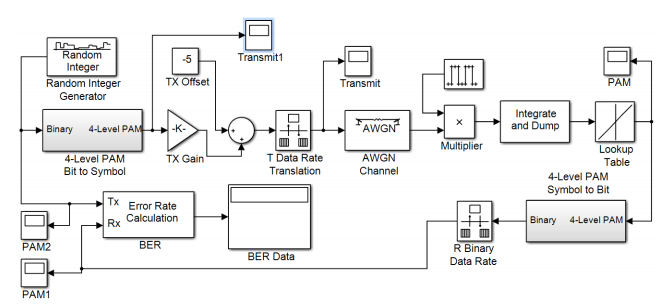
\includegraphics[scale=0.7]{fig1}
    \caption{Diagrama do sistema PAM.}
    \label{fig:1}
\end{figure}

Um sistema de comunicação digital PAM retangular M-ário com AWGN e um receptor ótimo implementado como um correlacionador é mostrado na figura \ref{fig:1}. Os pulsos 4-PAM retangular tem igual probabilidades a de ocorrências.

O próximo passo é montar um conversor binário de símbolos retangular conforme a figura \ref{fig:2}.
E também deve-se montar um conversor símbolos retangular para binário, conforme a figura \ref{fig:3}.

\begin{figure}[H]
    \centering
    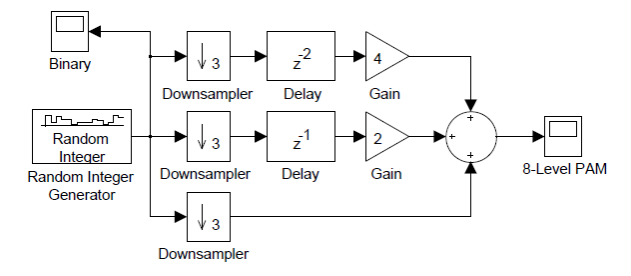
\includegraphics[scale=0.7]{fig2}
    \caption{Conversor de símbolos.}
    \label{fig:2}
\end{figure}

\begin{figure}[H]
    \centering
    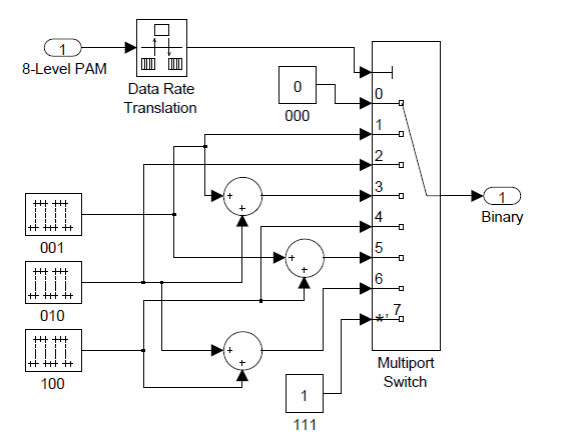
\includegraphics[scale=0.7]{fig3}
    \caption{Conversor de símbolos.}
    \label{fig:3}
\end{figure}

Em seguida, obter os gráficos nos pontos onde há osciloscópio  para o 4-PAM e também verificar o atraso no sinal recebido em relação ao transmitido. Plotar o gráfico BER x Eb/No (semilogy). 

Em seguida, montar uma tabela de acordo com a tabela \ref{tab:1}.

\begin{small}
    \begin{table}[H]
        \begin{center}
            \caption{Tabela BER x Eb/No}
            \begin{tabular}{c|c|c}
                \hline
                $\frac{Eb}{No}$ [dB] & BER & $P_b$ \\
                \hline
                $\infty$ & 0 & 0 \\
                \hline
                10 & & $2.4 \times 10^{-3} $\\
                \hline
                8 & $1.28 \times 10^{-3}$ & \\
                \hline
                6 & & \\
                \hline
                4 & & \\
                \hline
                2 & & \\
                \hline
                0 & & \\
                \hline
            \end{tabular}
            \label{tab:1}
        \end{center}
    \end{table}
\end{small}


\subsection{4-PAM com codificação Gray}
Como próxima atividade, simular o circuito 4-PAM com código Gray.

\begin{figure}[H]
    \centering
    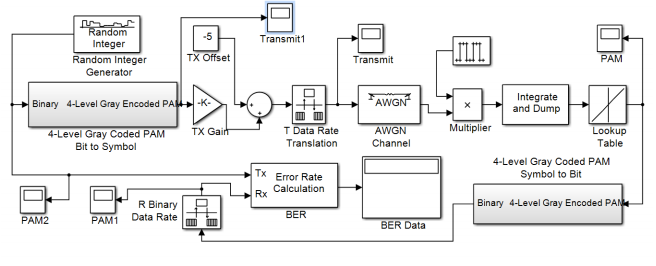
\includegraphics[scale=0.7]{fig4}
    \caption{PAM com código Gray.}
    \label{fig:4}
\end{figure}

O sistema de comunicação 4-PAM retangular e código Gray de 2 bits é similar ao sistema 4-PAM retangular não codificado. O código Gray atribuía entrada de di-bits 00, 01, 10 e 11 como os quatro níveis de saída 0, 1, 3 e 2 respectivamente.Os parâmetros de simulação devem ser ajustados de acordo com o roteiro.

Por conseguinte, gerar os gráficos nos pontos onde possui o osciloscópio BER. Verificar o atraso no sinal recebido em relação ao transmitido e plotar o gráfico BER x Eb/No (semilogy). A tabela \ref{tab:2} deverá ser preenchida com os dados encontrados. *Obs. A potência do sinal  é 13,9 W.

\begin{small}
    \begin{table}[H]
        \begin{center}
            \caption{Tabela BER x Eb/No para PAM com codificação Gray.}
            \begin{tabular}{c|c|c}
                \hline
                $\frac{Eb}{No}$ [dB] & BER & $P_b$ \\
                \hline
                $\infty$ & 0 & 0 \\
                \hline
                10 & & $1.8 \times 10^{-3}$\\
                \hline
                8 & $8.6 \times 10^{-3}$ & \\
                \hline
                6 & & \\
                \hline
                4 & & \\
                \hline
                2 & & \\
                \hline
                0 & & \\
                \hline
            \end{tabular}
            \label{tab:1}
        \end{center}
    \end{table}
\end{small}


E para finalizar, é necessário plotar em um mesmo gráfico as BER x Eb/No dos itens 2 e 4 do roteiro.
